% \documentclass[12pt,draftclsnofoot,peerreview,onecolumn]{IEEEtran}
\documentclass[journal,comsoc]{IEEEtran}
\usepackage[T1]{fontenc}
% \usepackage{cite}
% \usepackage{amsfonts}
\usepackage{amssymb}
\usepackage{amsmath}
\interdisplaylinepenalty=2500
\usepackage{filecontents}
\usepackage{url}
\usepackage{bm}
\usepackage[square,sort,comma,numbers]{natbib}
\usepackage{subfigure} 
% \usepackage{caption}
% \usepackage{subcaption}
\usepackage[colorlinks,
  linkcolor=black,
  anchorcolor=blue,
  citecolor=black
  ]{hyperref}
\ifCLASSINFOpdf
 \usepackage[pdftex]{graphicx}
\else
 \usepackage[dvips]{graphicx}
\fi

% correct bad hyphenation here
\hyphenation{op-tical net-works semi-conduc-tor}

\renewcommand{\citedash}{--}

\DeclareMathOperator*{\argmax}{arg\,max}

\begin{document}
%
% paper title
% can use linebreaks \\ within to get better formatting as desired

\title{Entropy Minimization Based Symbol Timing
\\and Carrier Frequency Recovery}
% \author{\IEEEauthorblockN{Xiao Liu and Jean-Fran\c{c}ois Bousquet }
% \IEEEauthorblockA{Electrical and Computer Engineering\\
% Dalhousie University\\
% Halifax, B3H 4R2, Canada\\
% Email: x.liu@dal.ca}}
\author{Xiao~Liu,~\IEEEmembership{Student Member,~IEEE,}
%         John~Doe,~\IEEEmembership{Fellow,~OSA,}
        and~Jean-Fran\c{c}ois~Bousquet,~\IEEEmembership{Member,~IEEE}% <-this % stops a space

\thanks{Manuscript received April 8, 2017; revised xxxx xx, 2017. This project was supported by the Atlantic Innovation Fund \#Project \#203162.}
\thanks{The authors are with the Department of Electrical and Computer Engineering, Dalhousie University, Halifax,
NS, B3J 1Z1, Canada (e-mail: \{x.liu, jbousquet\}@dal.ca).}% <-this % stops a space
% \thanks{J. Bousquet is with Dalhousie University.}% <-this % stops a space
}

% The paper headers
\markboth{IEEE Wireless Communications Letters,~Vol.~xx, No.~x, xxxxxx~2017}%
{Shell \MakeLowercase{\textit{et al.}}: Entropy Minimization Based Symbol Timing and Carrier Frequency Recovery}

% make the title area
\maketitle


\begin{abstract}
This paper  presents a new entropy minimization criterion that is used for both symbol timing and carrier frequency recovery in a wireless receiver.
It relies on the entropy estimation of the eye diagram and the constellation diagram of the received signal. 
During the parameter search, when the perfect synchronization is achieved, the entropy will reach a sharp global minimum, indicating the least intersymbol interference or a restored constellation diagram. 
% The minimized entropy indicates a regular pattern with the least interference, that is where the signal is synchronized and recovered correctly.
% In the synchronization parameter search, the corresponding entropy reaches a sharp global minimum when the signal is recovered correctly.
Unlike other synchronization methods, this unified criterion can be used to build an all-in-one synchronizer with high accuracy.
The feasibility of this method is proven using a theoretical analysis and supported with numerical simulation. 
\end{abstract}

% {\bf Keywords:} 
\begin{IEEEkeywords}
Entropy minimization, symbol timing, carrier frequency recovery, synchronization.
\end{IEEEkeywords}

\IEEEpeerreviewmaketitle

\section{Introduction}
\label{sec:intro}
\IEEEPARstart{I}{n} a digital receiver for wireless communication, 
the down-sampler is located after the matched filter.
It is triggered by a local clock to sample the filter output at multiples of the symbol period.
% In digital wireless communication systems, the bit streams we wish to transmit are inherently discrete-time signals while physical media are continuous-time in nature. 
% Therefore, the bit stream must be represented as a continuous-time signal for transmission.
% The most common solution is to apply pulse amplitude modulation (PAM).
% The bit stream is represented by pulses that are equally spaced in time with different amplitudes.
% The job of a receiver is to recover the transmitted symbols from the continuous-time signal.
% To that end, there is a down-sampler in the receiver that is triggered at multiples of the symbol period.
In the ideal case, the local clock is synchronized with the real symbol clock, however, since the symbol clock is usually unknown to the receiver, a symbol timing recovery circuit is required.
Particularly in a mobile channel, such as the underwater acoustic channel, the symbol clock period is time variant.
% In addition, for passband communication, the carrier frequency of the received signal may shift due to relative motion introduced by the Doppler effect.
In addition, the relative motion will shift the carrier frequency at passband, a phenomenon known as the Doppler shift. 
% Therefore a reliable synchronization circuit is in great demand.
Therefore a continuous estimation and compensation of the synchronization error is essential to maintain the link reliability.

The symbol clock has two fundamental parameters: symbol rate and symbol timing phase.
These parameters can be estimated either in feedback or feedforward configurations~\cite{mengali1997synchronization}.
% , \cite{meyr1997digital}. 
The feedback configuration features a timing error detector, 
that produces a signal proportional to the difference between the local timing phase and the actual symbol clock phase.
The filtered error signal is used to adjust the down-sampling clock with high accuracy.
On the other hand, the feedforward configuration can use a block of data to directly estimate the instantaneous timing offset to allow fast acquisition.
% has fast convergence speed. 
% a rapid acquisition, or in other words, high convergence speed. 
This paper is focused on the feedforward configuration to track rapidly changing propagation conditions.

Feedforward schemes recover the symbol clock by finding out the periodicity of the received time series signal.
To extract the frequency and phase of a periodic signal,
the Fourier analysis is the standard technique.
% \cite{oppenheim1997signals}.
% to apply Fourier Transform.
% The frequency and phase of the resulting spectrum peak(s) are the estimates.
However, it is not suitable for bandwidth efficient communication systems, 
particularly because the received signal is not periodic.
% nonstationary.
In these conditions, the square timing recovery method \cite{Oerder1988} is probably the most popular solution.
% method as a feedforward timing recovery method.
% This technique is based on applying a magnitude square to the received signal and extracting the timing phase from the spectral line at the symbol rate.
Indeed, since a linearly modulated waveform is second-order cyclostationary \cite{Gini1998}, the magnitude square can be considered as a second-order nonlinear transform.
As such, the square operation converts a cyclostationary signal into a periodic signal, such that the Fourier transform can be applied for symbol timing recovery.

% The continuous signal is pulse shaped to convey information within limited bandwidth. 
Since Shannon's work, entropy~\cite{Shannon1948} is used as a major tool in information theory. 
But except for theoretical analysis, it is rarely used in signal processing because of its complexity~\cite{Bercher2000}.
Nonetheless, it has been shown in~\cite{Pedzisz2006} that the carrier frequency offset of the \(M\)-ary PSK signals can be recovered by minimizing the entropy of the instantaneous phase probability density function.
Also, it has been reported that the error entropy minimization algorithms can be applied for channel equalization \cite{Santamaria2002}. 
However, no application can be found in the literature for symbol timing recovery.

In this paper, we propose a new synchronization criterion making use of the periodicity of the signal entropy.
The first advantage is that it can be applied to both symbol timing and carrier frequency recovery. 
% It can be applied to signal with linear modulation, and is not limited to constant envelop modulation.
Moreover, it only requires certain probability functions obtained from the eye diagram and constellation diagram, so the detectors described in this paper can also be used to track the clock during data detection. 
% In addition, the proposed method extracts information from the probability density function, so
In addition, entropy estimation measures intersymbol interference (ISI), and includes higher-order statistics of the data \cite{Santamaria2002}, whereas other m maximum likelihood based synchronization techniques only use second-order statistics and assume there is no ISI in the received signal~\cite{meyr1997digital}.
This is the underlying cause of its superior synchronization performance in distorted channels.

This paper is organized as follows.
In Section \ref{sec:timing}, the basics of information entropy are introduced and 
the entropy minimization criterion is discussed for symbol timing recovery.
Then it is applied to the complex signal for carrier frequency recovery in Section \ref{sec:carrier}.
% the case of complex signal and the carrier frequency recovery are illustrated 
The conclusion is presented in Section~\ref{sec:conc}.

\section{Timing Recovery Based on Entropy Minimization Criterion}
\label{sec:timing}
This section begins with the introduction of information entropy and how it is used to measure the randomness of the eye diagram. 
The system parameters and terminology are defined, 
and the algorithms that recover the symbol timing using the entropy of the eye diagram are detailed.
% The output of the entropy detector is used for symbol timing phase and symbol rate recovery.
% This section focuses on the theory, including the system parameters and terminology. 

\subsection{Entropy and System parameters}
\label{sec:entropy_assumption}
% In the late 1940's, Claude Shannon developed a mathematical theory of information \cite{Shannon1948}. 
The concept of entropy developed by Shannon is a measure of the amount of information or, in other words, its randomness.
% Intuitively, if a signal is random, that means its entropy is high, while a regular signal indicates its entropy is low.
Assuming \(k\) possible observations of a one-dimensional discrete signal,
with \(p_i\) representing the probability of the \(i\)-th possibility,
the information entropy \(H\) can be expressed as
\begin{equation}
% H =  - \sum {p_i}\log_2 {p_i},
H =  - \sum\limits_{i = 1}^k {{p_i}\log_2 {p_i}}.
\label{eq:entropy}
\end{equation}
Since the base of the logarithmic function is 2, 
the entropy is said to be in \textit{bits}.
% Note that \(p_i\) is the only argument in (\ref{eq:entropy}) denoting the probability of the \textit{i}-th possibility of variables.
% The number of possibilities is \(k\), however, for continues signal, \(k\) is the number of separations in amplitude.
The choice of \(k\) will affect the estimation of the entropy, which will be discussed later.

Before describing entropy based synchronization techniques,
% in Section \ref{sec:eye_entropy}, 
system parameters and terminology are defined here.
In this work, it is assumed that the signal is linearly modulated (not limited to phase-shift keying) with an alphabet size of \(M\).
The bit stream follows an independent identical distribution.
The pulse shaping filter is designed under the Nyquist criterion, such that there is no ISI at the proper sampling instances.
The span of the shaping filter is limited to \(L\) symbols, where \(L\) is an even number.
In this section, the channel distortion is neglected, the symbol rate is known and the signal is analyzed at baseband without carrier frequency offset.
Some of these system parameters will be reviewed in the next few sections.

% Seven assumptions are made before the future study on the entropy based synchronization techniques:
% \begin{enumerate}
% \item The signal is linear modulated (not limited to constant envelope modulation) with a alphabet size of \(M\).
% \item The bit stream has independent identical distribution.
% \item The pulses are designed under Nyquist criterion, which means there is no intersymbol interference (ISI) at the proper sampling instances.
% \item The pulses are truncated to \(N\) symbols, where \(N\) is an even number.
% \item The channel distortions are neglected.
% \item The symbol rate is known.
% \item The communication is in baseband.
% \end{enumerate}
% Note that some assumptions will come loose in the future discussion.

\subsection{Eye Diagram Entropy and Timing Phase Search}
\label{sec:eye_entropy}
The eye diagram is a graphical illustration that consists of many overlaid traces of small sections of a signal. 
Normally, the length of the window is one or two symbol periods. The ideal down-sampling instant is located in the middle of the eye diagram where the eye opening reaches its maximum, indicating the optimum error immunity.
Fig. \ref{fig:eyediagram} is an eye diagram for a BPSK signal overlaid at each symbol period.
The binary data is shaped using raised-cosine pulses with a roll-off factor of 0.5.

% With the system described in Section \ref{sec:entropy_assumption},
Since the data is equally distributed in \(M\) possible symbols, 
the probability of the $i$th entropy is \(p_i=1/M\) and $k$ is equal to $M$.
% It is easy to infer from (\ref{eq:entropy}) that 
Substituting this in~(\ref{eq:entropy}), the entropy in the middle of the eye,
i.e., the amount of information carried by each symbol, is given by
\begin{equation}
H_{mid} =  - \sum\limits_{i = 1}^M {{\frac{1}{M}}\log_2 {\frac{1}{M}}}=\log_2 {M}.
\label{eq:entropy_mid}
\end{equation}
According to the Nyquist criterion, there is no ISI in the middle of the eye diagram, so the alphabet size \(M\) is the only unknown parameter in (\ref{eq:entropy_mid}).
However, there are \(L\) adjacent pulses that interfere with each other in its neighbouring area,
so the maximum accumulated information entropy is up to
% while its neighbouring entropy is
\begin{equation}
H_{neb} =  L\log_2 {M}.
\label{eq:entropy_neb}
\end{equation}
% The extra information in the neighbouring area is due to the ISI from adjacent pulses.
% According to the Nyquist criterion,
Since only the proper sampling instances are ISI free,
one can conclude that the entropy of an eye diagram comes to a global minimum in the middle of the eye. 

\begin{figure}[htbp]
\centering
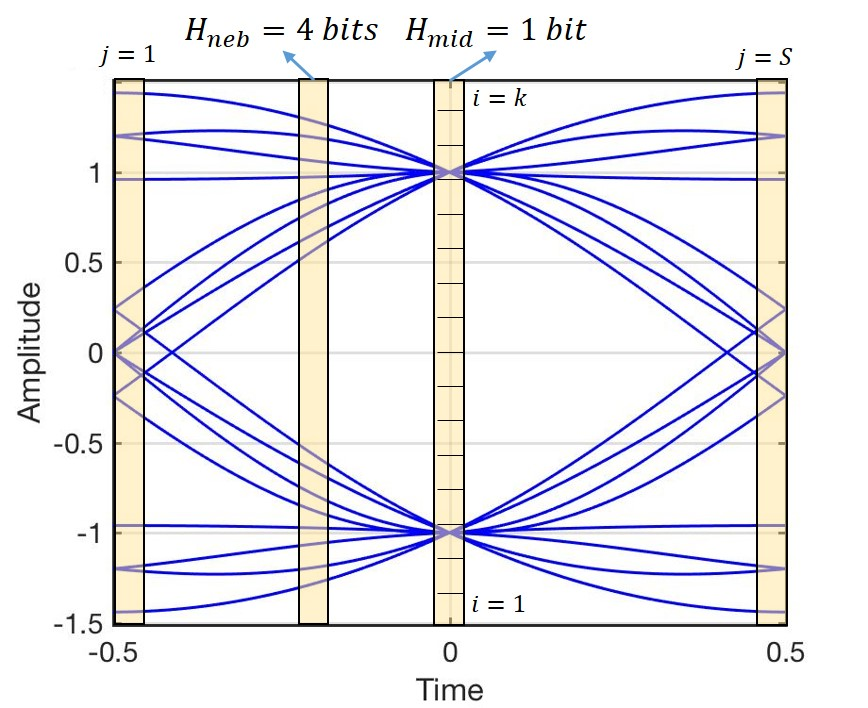
\includegraphics[width=2.5in]{sym_rate_right3.jpg}
\caption{Eye diagrams of a BPSK signal and its timing phase entropy.}
\label{fig:eyediagram} 
\end{figure}


For example, Fig. \ref{fig:eyediagram} is an eye diagram of a BPSK signal ($M=2$), where \(L=4\). 
In the middle of the eye, i.e., at instant $t=0$, the entropy \(H_{mid} = \log_2 2 = 1\)~bit, 
while its neighbouring entropy \(H_{neb} = 4\log_2 2 = 4\) bits.
In other words, the entropy of the optimum symbol timing phase is significantly lower than in its neighbouring area.


% \label{sec:phase_evaluation}
% 采样,精度
Next, let's consider some practical issues and test this criterion with numerical simulations.
For low symbol rate communication, such as underwater acoustic applications, 
it is reasonable to assume that the sample rate of the receiver's analog to digital converter (ADC) is much higher than the symbol rate, so that the down sampling can be realized using 
decimation instead of interpolating.
% picking up a sample instead of interpolation.
% Moreover, we will follow the same order in Section \ref{sec:theory} that first
% focusing on the timing phase recovery by assuming the symbol rate is known, and then expand it to the symbol rate estimation.

%  m*n matrix
If a block of  samples under observation consists of \(N\) symbols and the oversampling rate is \(S\) samples per symbol,
the eye diagram data can be constructed by reshaping the samples into an \(N\) by \(S\) matrix.
The one-dimensional \textit{timing phase entropy} is found with the \(N\) samples in column \(j\) (the yellow column in Fig.~\ref{fig:eyediagram}), where \(1 \le j \le S\). 
The peak-to-peak amplitude of the samples is partitioned into \(k\) bins and the entropy at the timing phase index \(j\) is given by 
% the equation similar to (\ref{eq:entropy}):
\begin{equation}
H_j =  - \sum\limits_{i = 1}^k {\frac{l_{i,j}}{N}\log_2 \frac{l_{i,j}}{N}},
\label{eq:entropy_phase}
\end{equation}
where \(l_{i,j}\) is defined as the number of samples falling in the \(i\)-th (\(1 \le i \le k\)) partition at phase index $j$. 


The upper limit of number of partitions \(k\) is decided by the ADC's quantization resolution.
% or its truncation result.
The values are usually in binary form, so the resolution is usually expressed in bits too.
Therefore, the number of output discrete values available (partitions) is expected to be a power of two. 
For example, an ADC with a resolution of 8 bits can encode an analog input to 256 different partitions, since \(2^8 = 256\). 

To illustrate the influence of the number of partitions, 
the entropy is plotted as a function of symbol timing phase for different ADC resolutions in Fig. \ref{fig:phase_entropy}.
The entropy is calculated from the signal in Fig. \ref{fig:eyediagram}.
The partitions are chosen for an ADC with a resolution from 4 to 7 bits,
and the corresponding numbers of partitions are 16, 32, 64 and 128.
In the figure, the entropy reaches a global minimum of 1 bit when the timing phase offset is 0, and the entropy in the neighbouring area is as high as nearly 4 bits for higher numbers of partition. 
These results confirm the expected value obtained from (\ref{eq:entropy_mid}) and (\ref{eq:entropy_neb}).
% agree with the conclusion drawn in Fig. \ref{fig:eyediagram}.
It can be observed that the more partitions used in the entropy estimation, the sharper the entropy groove will be.
The increased number of partitions can improve the timing phase estimation accuracy, but increases the computational complexity in the same time.
% is rather complex from the computational point of view.

\begin{figure}[htbp]
\centering
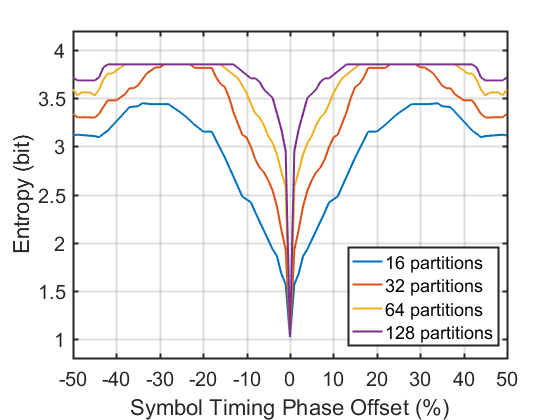
\includegraphics[width=2.5in]{phase_entropy.png}
\caption{Symbol timing phase entropy (with smoothing) for different number of partitions.}
\label{fig:phase_entropy} 
\end{figure}
One can notice that in Fig. \ref{fig:phase_entropy}, there are  local minima when the timing phase offset is at 50\%.
This is due to the zero-crossing caused by symbol transitions.
The local minima indicate that a simple gradient descent algorithm may not be suited for this application, while a global search is a slow yet safe way to find the minimum.
% Alternatively, during the entropy calculation, samples with its value close to zero can be neglected to reduce the entropy contribution. 



\subsection{Symbol Rate Search}
\label{sec:symbol_rate}
Timing phase estimation is achieved by searching the minimized timing phase entropy of the eye diagram,
while the symbol rate search needs to minimize the entropy of the whole eye diagram.
The \textit{eye diagram entropy} is given by integrating the timing phase entropy of all the \(S\) columns in the eye diagram.
% According to Section \ref{sec:symbol_rate}, the eye diagram entropy is defined by
% Note that the symbol rate is unknown right now, so \(S\) is a trial number of samples per symbol.
The eye diagram entropy is written as
\begin{equation}
H_{eye} =   \sum\limits_{j = 1}^S {H_j}.
\label{eq:entropy_rate}
\end{equation}
In (\ref{eq:entropy_rate}), the timing phase entropy \(H_j\) is integrated through the eye diagram.
Thus $H_{eye}$ can be considered as a two-dimensional entropy.


% If we remove the assumption 6) in Section \ref{sec:entropy_assumption},
For example, even if there is 1\% symbol rate error, the eye diagram in Fig. \ref{fig:eyediagram} will be completely closed.
% as shown in Fig. \ref{fig:eyediagram_rate}.
% Fig. \ref{fig:eyediagram} is redraw with 1\% symbol rate error, and we have Fig. \ref{fig:eyediagram_rate}.
The solution for the eye diagram entropy with symbol rate error is hard to solve analytically, 
but it is obvious that there is much more ISI or randomness throughout all the timing phases than that in Fig.~\ref{fig:eyediagram}.
% Therefore, only when the symbol rate is restored, will the eye diagram come to its most open state and its entropy will reach to its minimum.
Therefore, only when the symbol rate is restored does the eye diagram become open, and correspondingly the entropy reaches its minimum.

% \begin{figure}[htbp]
% \centering
% 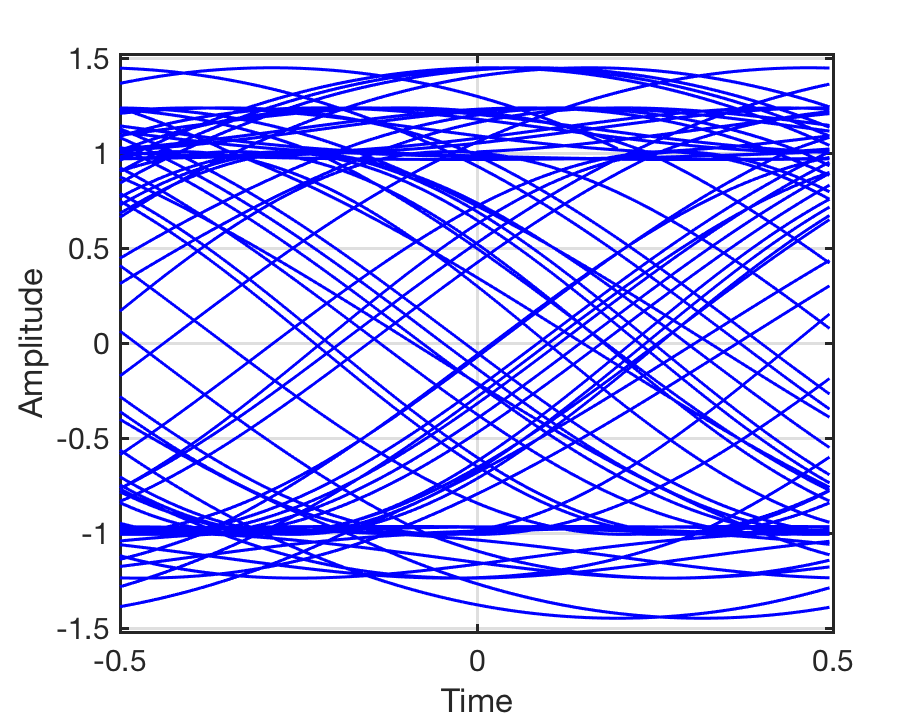
\includegraphics[width=2.5in]{sym_rate_wrong3.png}
% \caption{Eye diagrams with 1\% symbol rate error.}
% \label{fig:eyediagram_rate} 
% \end{figure}

% \subsection{Symbol Rate Estimation}

The idea symbol rate search is equivalent to the estimation of the actual oversampling rate \(S\).
For demonstration purposes, \(S\) is set to a very high value of 200, so that the symbol rate  error can be as small as 0.5\% by an integer  oversampling rate estimate \(\hat S\).
In the simulation, \(\hat S\) ranges from  \(S-6\) to  \(S+6\), representing a symbol rate error from -3\% to 3\%.
All other system parameters are set as defined in Section \ref{sec:eye_entropy}. 
The eye diagram entropy is numerically calculated using (\ref{eq:entropy_rate}) and the results are plotted as a function of symbol rate error for different number of partitions in Fig. \ref{fig:rate_entropy}.
The value of the entropy reaches a sharp minimum when the symbol rate trial \(\hat S\) is equal to \(S\).
Similar to the timing phase entropy plot, more partitions lead to a deeper groove, but outside the groove, the eye diagram entropy curve is almost flat.
% The drop of the eye diagram entropy becomes dramatic with the increase of the number of partitions.
% Beyond the symbol rate error free zone, unlike the case for timing phase entropy, the eye diagram entropy curve is almost flat.
% making it difficult to apply gradient descent algorithm for symbol rate  search.

\begin{figure}[htbp]
\centering
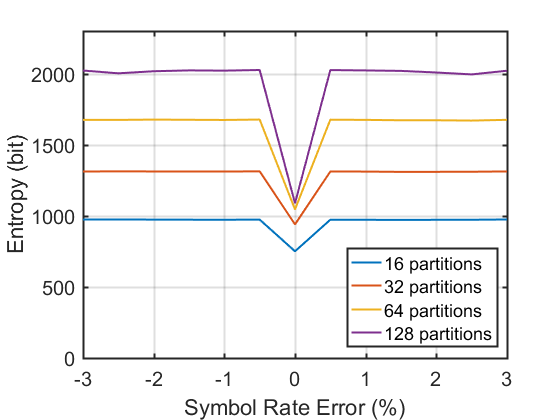
\includegraphics[width=2.5in]{rate_entropy.png}
\caption{Eye diagram entropy for different symbol rate estimation.}
\label{fig:rate_entropy} 
\end{figure}
In the entropy calculation for both symbol timing phase and symbol rate search, 
the algorithm requires \(N\) symbols to generate one entropy result.
Since the entropy is a function of probability, to obtain relative accurate probabilities, \(N\) cannot be set to a small value.
% Regarding the number of symbols \(n\), it does not affect the entropy calculation a lot in both symbol timing phase and symbol rate search.
In the simulation, the results tend to be stable when \(N\) is greater than a few hundreds symbols.
Below that number, the probability function may have significant bias.
% For this reason, the current algorithm works block by block, which is different from other feedback algorithms.

\section{Complex Signal and Carrier Frequency Recovery}
\label{sec:carrier}


In this section, the complex signal at baseband with in-phase and quadrature~(I/Q) components is considered.
The carrier frequency offset can introduce rotation of the complex signal in the constellation diagram.
It will be shown in this section that such frequency offset can be recovered by a similar entropy minimization criterion with the help of the constellation diagram.
% Also an entropy minimization based algorithm is applied to compensate for the carrier frequency offset.
% due to the down-conversion from the passband to the baseband.
% The carrier frequency offset can introduce rotation of the I/Q signal in the constellation diagram,
% and as will be shown that it can be recovered by a similar entropy minimization criterion.
% the assumption 7) in in Section \ref{sec:entropy_assumption} is extended to passband.
% the in-phase and quadrature~(IQ) components after down conversion are considered and the carrier frequency offset will also be included. 
\subsection{Entropy of Complex Signal}
When converted to baseband, the signals from in-phase and quadrature channel can generate two independent eye diagrams.
However, if we consider the I/Q components as one complex signal, the two eye diagrams can be combined to generate a new Cartesian plot.
% One way to calculate the entropy is to combine the two eye diagrams into one with the same time axis.
% Such method will add 1 bit to both \(H_{mid}\) and \(H_{neb}\), 
% but it doesn't change the  entropy difference (\(H_{neb}-H_{mid}\)).
% and there will be no change in the resulting entropy difference (\(H_{near}-H_{mid}\)).
% To increase the processing gain brought by the additional alphabet size, the I/Q components need to be processed jointly.
% The two sets of data are packaged into one complex data stream, or in other words, the complex envelope.
% In the meantime, the eye diagram is extended to be three-dimensional.
For each symbol timing phase, instead of a set of scalars representing the signal amplitude, it is a set of complex data containing both the in-phase data on the real axis and the quadrature data on the imaginary axis.
In fact, a diagram of such a set of complex data can be represented using a constellation diagram.

The \textit{constellation diagram entropy} is an extension of the timing phase entropy discussed in Section \ref{sec:eye_entropy}.
% It is a function of both timing phase \(j\)  and carrier frequency offset \(\Delta f\).
To estimate its value, the constellation diagram is partitioned into a matrix of \(k\) by \(k\) bins.
Fig. \ref{fig:const_entropy} is an example showing the partition of a constellation diagram with perfect symbol timing recovery but small carrier frequency offset \(\Delta f\). 
In this figure, \(k=16\) and  the coordinate of the yellow bin is (7, 15).
For \(N\) symbols under observation, if there are \(l_{xy}\) samples falling into bin ($x, y$), the constellation diagram entropy is given by
\begin{equation}
H_{\Delta f} =  -\sum\limits_{x=1}^k \sum\limits_{y = 1}^k {\frac{l_{xy}}{N}\log_2 \frac{l_{xy}}{N}}.
\label{eq:entropy_const}
\end{equation}
\begin{figure}[htbp]
\centering
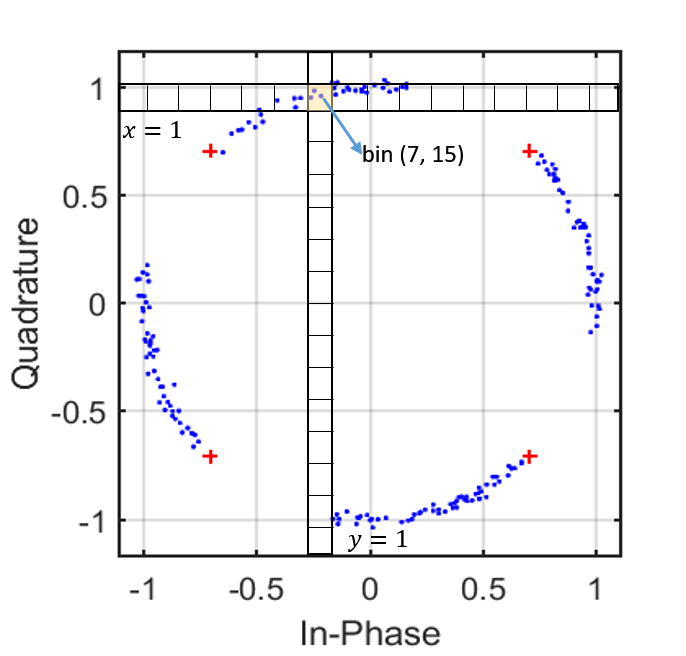
\includegraphics[width=2.5in]{const_ent.png}
\caption{Constellation diagram of a QPSK signal with carrier frequency offset and its partitions for entropy estimation.}
\label{fig:const_entropy} 
\end{figure}
% Its value can be found by partitioning the constellation diagram into \(k\) by \(k\) bins, 
% and then using a similar procedure shown in Section \ref{sec:symbol_rate}, 
% since the techniques essentially involve finding the entropy of a set of two-dimensional data.

% More details on the algorithms are discussed in Section \ref{sec:algorithm}.

% Using this method, the ideal entropy in the middle of the eye and its neighbouring area can be estimated by the same equations as (\ref{eq:entropy_mid}) and (\ref{eq:entropy_neb}).
% That means from the entropy perspective, there is no difference between the PAM and I/Q modulations with same alphabet size \(M\). 

\subsection{Frequency Offset Search}
The most notable synchronization issue that is unique in passband communication is the carrier frequency recovery.
It originates because of the the frequency difference between the carrier of the received signal and the local down converter.
It has been mentioned in Section \ref{sec:intro} that the entropy of the instantaneous phase probability density function can be used for carrier frequency recovery.
In fact, the carrier frequency can also be restored by minimizing the constellation diagram entropy. 
Unlike the symbol timing recovery, the extra entropy when there is frequency offset is mainly from the rotating constellation.
That is to say, by applying the entropy minimization criterion, both symbol timing and carrier frequency can be recovered.
Therefore, an all-in-one synchronizer can be designed based on one single criterion.

% \section{Simulation and Verification}
% \label{sec:simulation}
% In this section the entropy minimization principle is tested for both symbol timing and carrier frequency offset recovery. 
% Details on the algorithms are given, and the choice of parameters is discussed.



To verify the constellation diagram entropy based carrier frequency offset search, a simulation is run.
The modulation scheme is QPSK with \(\pi/4\) phase offset.
% , which can be considered as 2 BPSK streams composed of I/Q components.
In this example, the carrier frequency offset ranges from -3\% to 3\% of the symbol rate.
The constellation diagram entropy is taken in the centre of the eye diagram for each frequency offset setting.
The results are shown in Fig. \ref{fig:carrier_entropy}.

\begin{figure}[htbp]
\centering
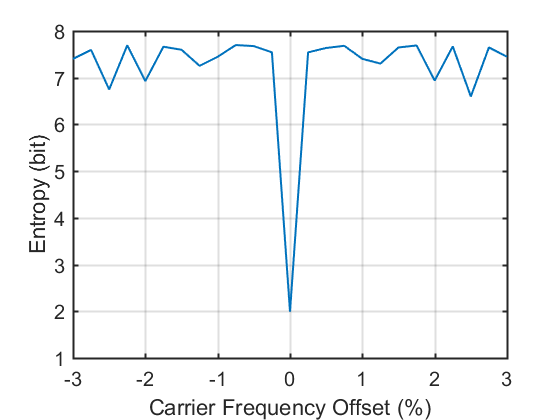
\includegraphics[width=2.5in]{carrier_entropy.png}
\caption{Constellation diagram entropy as a function of frequency offset.}
\label{fig:carrier_entropy} 
\end{figure}

In this figure, the constellation diagram entropy reaches a global minimum when the carrier frequency offset is 0.
Unlike Fig. \ref{fig:phase_entropy}, The minimum entropy here is 2 bits.
That is because the alphabet size for QPSK modulation is 4 and according to~(\ref{eq:entropy}) the resulting entropy is \(\log_2 {4}=2\) bits.
As such it can be observed that a global minimum is reached using entropy minimization for carrier frequency recovery as well as symbol timing recovery. 
% This figure and Fig.~\ref{fig:phase_entropy}, Fig.~\ref{fig:rate_entropy} have one thing in common, 
% that is when the received signal is perfectly synchronized, the corresponding entropy reaches a sharp global minimum.
% It proves that both symbol timing and carrier frequency recovery can be solved under one unified entropy minimization criterion.

\section{Conclusion Remarks}
\label{sec:conc}
A new unified synchronization criterion for wireless coherent communication, i.e., entropy minimization, has been investigated in this paper. 
The entropy of the received signal's eye diagram and constellation diagram is utilized to recover both symbol timing and carrier frequency offset.
In contrast to the widely used maximum likelihood based synchronization techniques, it is expected to achieve better performance due to the use of higher-order statistics.
% In an eye diagram, a perfect symbol timing is where there is no ISI, and in a constellation diagram, the carrier frequency is recovered when it stops rotating.
% Both the ISI and constellation rotation can introduce randomness,
% and since the entropy is a measure of randomness, 
% it can be used as a criterion to search for the synchronization parameters.
During the parameter search, when the perfect synchronization is achieved, the entropy will reach a sharp global minimum, indicating an open eye diagram or restored constellation. 
Therefore, an all-in-one synchronizer can be designed based on this one criterion alone. 

% However, the calculation of entropy and the global search algorithm are rather complex from the computational point of view.
Because the global search algorithm requires significant hardware complexity, it can be best implemented on embedded processors with massive parallel computation capability, such as FPGAs.  
% Also, to implement a clock and data recovery in realistic wideband environments, the algorithm must be improved in the presence of multipath arrival.  
A computationally efficient algorithm and its performance in a distorted channel should be considered for system implementation applied to realistic wideband wireless channels.
% criterion, principle, method, approach, algorithm



% \section*{Acknowledgement}
% The authors would like to thank Atlantic Canada Opportunities Agency
%  for financial support. 

\small
\bibliographystyle{IEEEbib}
\bibliography{Mendeley}


\end{document}